
\textcolor{red}{[$g_A(0)$ challenges history, excited states]}

Computations of the nucleon axial charge have long been considered
 a vital benchmark for nucleon physics with lattice QCD.
This quantity has been precisely measured with experiments probing neutron beta decay,
 characterized by a weak decay with a low momentum transfer.
Historically, lattice calculations of the axial charge have obtained values
 that were $O(10\%)$ too low, despite significant investments of effort.
This has been the subject of some controversy,
 with more and more sophisticated calculations to scrutinize lattice systematics.
Over time, contamination from excited states was identified as
 an important contributing factor to the systematic deviation.
Many collaborations have opted for high-statistics computations
 to reduce the statistical uncertainty at late times and permit
 multi-exponential fits to the time dependence of the correlation functions.
As time progressed, LQCD results moved closer to the experimental value,
 and now modern calculations are in agreement with experiment
 at the 1\% level~\cite{Kronfeld:2019nfb}.
\textcolor{red}{[more citations]}
Modern efforts to compute nucleon matrix elements now target the nucleon
 axial form factor with its four-momentum transfer dependence.

To check the accuracy of lattice QCD calculations targeting the axial form factor,
 the validity of the partially-conserved axial current (PCAC) relation,
\begin{align}
 \partial^\mu A^{a}_{\mu}(x) = 2 m_q P^{a}(x),
 \label{eq:pcac}
\end{align}
 has been scrutinized with lattice data.
The PCAC relation is an exact symmetry in the continuum limit.
The generalization of this relation to the nucleon form factors
 yields the generalized Goldberger-Triemann (GGT) relation,
\begin{align}
 2 M_N G_A(Q^2) -\frac{Q^2}{2M_N} \widetilde{G}_P(Q^2) = 2 m_q G_{P}(Q^2),
 \label{eq:ggt}
\end{align}
 which provides orthogonal checks of individual matrix elements
 for the axial and pseudoscalar currents.
The pion pole dominance (PPD) ansatz is also studied,
\begin{align}
 \widetilde{G}^{\rm PPD}_P(Q^2) = \frac{4M_N^2}{Q^2+M_\pi^2} G_A(Q^2),
 \label{eq:ppd}
\end{align}
 which is only approximate even in the continuum and is obtained
 by carefully considering the leading asymptotic behavior of the
 form factors in the double limit $Q^2\to0$ and $m_q\to0$~\cite{Sasaki:2007gw}.

Initial calculations targeting the axial form factor verified the PCAC relation
 for the full correlation functions but found significant \emph{apparent} violations
 of the Generalized Goldberger-Triemann relation, Eq.~\ref{eq:ggt}.
The resolution of the apparent violation of GGT
 is now informed by baryon chiral perturbation theory, which suggests that chiral
 and excited state corrections to the spatial axial, temporal axial, and induced pseudoscalar
 are functionally different and not properly removed.
The axial contributions are largely dominated by $N\pi$ excited states
 with a highly suppressed single nucleon chiral correction.
The correction to the axial current is nearly independent of $Q^2$.
On the other hand, corrections to the induced pseudoscalar are
 driven by the single nucleon chiral contribution and has
 a strong $Q^2$ dependence~\cite{Bar:2018xyi}, with the largest correction at low $Q^2$.
The $N\pi$ contribution in the induced pseudoscalar is highly suppressed by
 an approximate cancellation.
The contamination to the pseudoscalar current is redundant with the
 axial and induced pseudoscalar chiral corrections and can be obtained
 by application of the PCAC relation.

Scrutiny of the lattice QCD data has demonstrated many of the features
 that were expected from chiral perturbation theory.
The primary excited state contaminations to the axial matrix elements
 were shown to be driven by two specific $N\pi$ states,
 characterized by a transition through an axial current
 of the nucleon state to an $N\pi$ excited state or vise versa~\cite{Jang:2019vkm}.
\textcolor{red}{[is below statement understandable?]}
The momenta of the states with the strongest contribution are those
 where a valence quark diagrams can be drawn containing only a single
 zero-momentum gluon emission, which fixes the relative momenta of the
 quark constituents making up the nucleons and the pion.
These $N\pi$ states were initially expected to be negligible due to a volume suppression
 of the state overlap, which makes them invisible to the two-point functions~\cite{Bar:2016uoj}.
However, the three-point axial matrix element enhances these contributions relative
 to the ground state nucleon matrix element, which is enough to overcome the volume suppression.
As a consequence, analyses that fix the spectrum using the two-point functions alone
 will often miss the important $N\pi$ contamination to the
 axial matrix element~\cite{Jang:2019vkm,He:2021yvm}.

The lattice data also showed deviations as large as $40\%$ from the pion pole
 dominance ansatz at low $Q^2$, where it was expected to
 work best~\cite{Bali:2014nma,Gupta:2017dwj}.
Each $Q^2$ prefered dominant $N\pi$ states with different energies,
 which when neglected across the full range of momentum transfers
 produced a $Q^2$-dependent discrepancy in excess of the $Q^2$ behavior
 expected from the GGT and PPD relations.
Fits to the three-point functions that allow for the possibility of
 nonnegligible $N\pi$ states are able to constrain the effects of these states,
 removing the contamination and thereby restoring the PPD relation.

\textcolor{red}{[NME]}
\textcolor{red}{[RQCD]}

\textcolor{red}{[ETMC]}
The ETMC calculation~\cite{Alexandrou:2020okk} of the axial form factor
 is performed on three ensembles with twisted mass fermions all at physical pion mass.
Two of these ensembles include only light quarks in the sea,
 leading to unquantifiable systematic corrections from
 neglecting the effects of strange quarks.
However, these two two-flavor ensembles permit an explicit test of finite-volume corrections,
 demonstrating a lack of dependence on the volume in the range of typical lattice computations.
The remaining ensemble has four flavors of sea quarks and thus is not subject
 to the same criticism of neglecting the strange quarks.
Despite the agreement with the trend of axial form factor results from other collaborations,
 the results from this computation do not satisfy the PPD and GGT relations,
 suggesting remnant excited state contamination.

\textcolor{red}{[PACS]}
The PACS collaboration has focused on computing the axial form factor
 on large ensembles with Wilson clover fermions at
 physical pion mass~\cite{Ishikawa:2018rew,Shintani:2018ozy}.
The ensemble used in this analysis has a volume of $(10.8~{\rm fm})^3$,
 considerably larger than ensembles used by other collaborations.
The large volume reduces the minimum $Q^2$ that can be probed
 with the discrete lattice momenta but forces the need for many units of momenta
 to access the same kinematic range as other computations.
They compare this ensemble to a computation of the axial radius using
 the traditional method compared with derivatives obtained from
 moments of the correlators~\cite{Aglietti:1994nx},
 on a $(5.5~{\rm fm})^3$ volume ensemble, finding agreement between the results of each.
Results on both ensembles are about $1\sigma$ small compared to the axial radius
 from the average from experimental sources in Ref.~\cite{Hill:2017wgb}.
Like the ETMC results, the PACS calculation does not satisfy the PPD and GGT relations.

\textcolor{red}{[CLS]}
The CLS collaboration have an axial form factor computation on a
 single ensemble of Wilson clover fermions at physical pion mass~\cite{Hasan:2017wwt}.
This methodology paper focuses on computing the nucleon charges
 and radii by explicitly computing derivatives of the correlation functions
 with respect to the momentum transfer.
This method yields the axial radius directly from $Q^2=0$ data,
 which is compared to the nucleon form factor slopes and charges obtained from
 fits to data at nonzero $Q^2$ using the traditional three-point correlator methods.
Though the results are in agreement between the two methods,
 the direct derivative proves to be noisier than the traditional method.
With more precision, the axial radius obtained from this method,
 or constraints on the slope obtained in a similar fashion at nonzero $Q^2$,
 could provide orthogonal constraints on the form factor that could
 help pin down the axial form factor shape.

\textcolor{red}{[Other calculations]}
In addition to the aforementioned published results,
 a handful of recent preliminary results that deserve mention.
The Mainz collaboration has an ongoing calculation on 12 ensembles,
 including an ensemble at physical pion mass
 and a chiral-continuum and infinite volume extrapolation~\cite{Djukanovic:2021yqg}.
This computation is performed with improved Wilson fermions.
The Fermilab Lattice and MILC collaborations also have an ongoing
 computation of the axial form factor using a unitary HISQ-on-HISQ setup,
 for which a preliminary computation of the axial charge on
 a single unphysical ensemble exists~\cite{Lin:2020wko}.
Because of the choice of action, this computation has more nucleon ``tastes''
 than other efforts, which is more computationally affordable
 at the cost of a more challenging analysis.
The CalLat collaboration have a computation of the axial form factor
 using a mixed-action domain wall on HISQ setup,
 with existing data on several ensembles including multiple physical pion mass ensembles.
The fits to one physical mass ensemble from the CalLat collaboration are used
 to make statements about the pheno impact of the LQCD results in Sec.~\ref{sec:impact}.

\begin{figure}[hbt!]
\centering
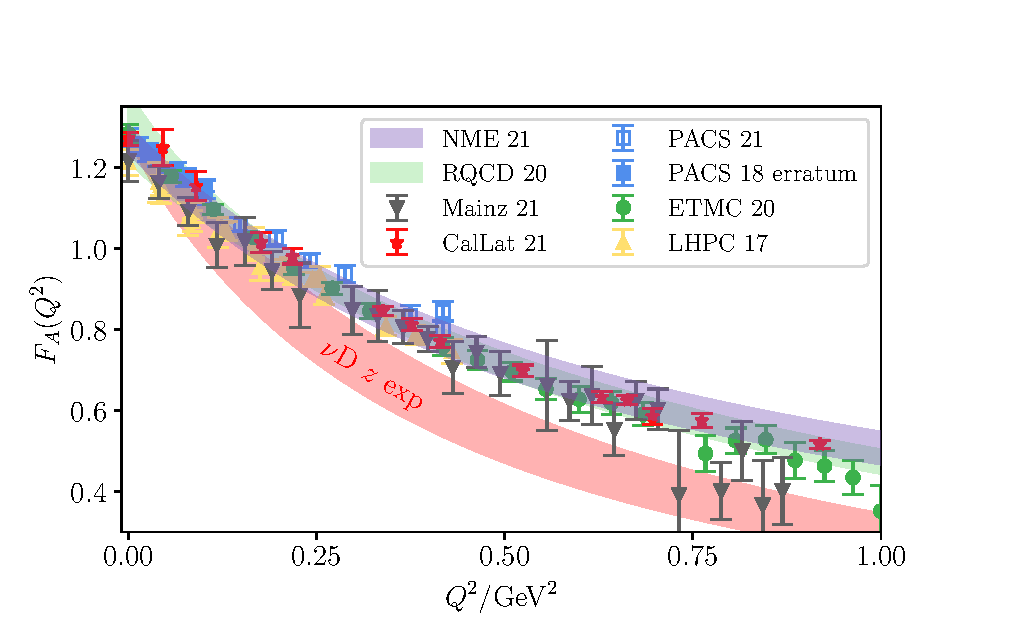
\includegraphics[width=0.5\textwidth]{plots/gaq2-overlay-standalone.pdf}
\caption{
Published results for the axial form factor obtained from lattice QCD,
 compared with the deuterium extraction from Ref.~\cite{Meyer:2016oeg}.
Collaborations that have obtained their results from only a single ensemble
 are plotted as scatter points.
These single-ensemble results will have small but unknown corrections due to chiral, continuum,
 and finite volume systematic shifts.
The NME~\cite{Park:2021ypf} and RQCD~\cite{RQCD:2019jai}
 results are both obtained from fits to several ensembles.
The RQCD perform the full chiral-continuum and finite volume extrapolations to the data,
 fitting to each of the form factors independently for each ensemble but providing
 the constraint that the form factors must satisfy the GGT relation in the continuum.
The NME collaboration also performed a chiral-continuum and finite volume extrapolation
 on their data, but found significantly larger uncertainties and so their result
 is obtained from an average of the results on their five largest volume ensembles.
As a rough estimate, NME claims that the uncertainties are at least a factor of 5 larger
 if the fits are relaxed to allow the results to change with pion mass or lattice spacing.
}
\end{figure}

\begin{itemize}
\item
\textcolor{red}{[
 temporal axial current - subject to large excited state corrections.
 ETMC claim precise, use it to constrain $N\pi$.
]}
\item
\textcolor{red}{[
 Axial form factor has different corrections than induced pseudoscalar.
 Most of $N\pi$ contamination introduced into GGT and PCAC from induced pseudoscalar.
]}
\item
\textcolor{red}{[ ensemble details of calculations.]}
\item
\textcolor{red}{[
 $g_A(Q^2)$ parameterizations.
 $z$ expansion intro, taken from chiral section.
]}
\item
\textcolor{red}{[
 Different methods of dealing with excited states.
 FH, 3pt fits, summation, other?
]}
\item
\textcolor{red}{[
 axial form factor with full set of coefficients and covariance needed
 in chiral-continuum-FV limit.
 $r_A^2$ reported to connect with pion electroproduction/neutron decay/very low-$Q^2$ applications,
 but not nearly as important for neutrinos.
]}
\item
\textcolor{red}{[ Need an axial ff calculation with explicit $N\pi$-like operators. ]}
\item
\textcolor{red}{[ Will need to verify systematics for large $Q^2$ axial ff,
 but chiral corrections/excited state contaminations are also smallest in this region.
 May be fooled into comfort by breakdown of XPT.
]}
\item
\item
\textcolor{red}{[
 failure of dipole parameterization with existing LQCD data.
 consistency with expt for $r_A^2$ but high at large $Q^2$ means
 that one-parameter fits are insufficient to describe $Q^2$ behavior.
 ]}
\end{itemize}

Citations for $F_A(Q^2)$ references pulled from NME21, no $g_A$-only references:
\begin{description}
\item[NME 21]~\cite{Park:2021ypf}
\item[RQCD 20]~\cite{Bali:2018qus,RQCD:2019jai} %% 63
\item[ETMC 20]~\cite{Alexandrou:2018sjm,Alexandrou:2019brg,Alexandrou:2020okk} %% 54-56
\item[PACS 18 (erratum)]~\cite{Ishikawa:2018rew,Shintani:2018ozy} %% 60-61 (62 proceedings)
\item[PNDME 17]~\cite{Gupta:2017dwj,Gupta:2018qil,Jang:2019vkm,Jang:2019jkn} %% 6-9
\item[CLS 17]~\cite{Hasan:2017wwt,Hasan:2019noy} %% LHPC? 66-67
\end{description}
Other axial ff effort references:
\begin{description}
\item[new PACS gA(Q2)]~\cite{Ishikawa:2021eut}
\item[Mainz gA(Q2)]~\cite{Djukanovic:2021yqg}
\item[Fermilab Lattice+MILC HISQ gA(0)]~\cite{Lin:2020wko}
\item[CalLat gA(Q2)]~\cite{Meyer:2021vfq}
\end{description}
Other references:
\begin{description}
\item[USQCD white paper]~\cite{Kronfeld:2019nfb}
\item[FLAG 21]~\cite{Aoki:2021kgd}
\item[CalLat excited states $g_A$]~\cite{He:2021yvm}
\item[Ottnad excited states]~\cite{Ottnad:2020qbw}
\item[Baer XPT]~\cite{Bar:2018xyi,Bar:2019igf}
\item[Axial radius from LQCD using XPT]~\cite{Yao:2017fym}
\end{description}

